% ============================================================
%  The Particle Model — Lesson Booklet (one section per lesson: A Reading · B Theory · C Practice · D Above level)
%  Year 7 (Year 8 extension)  |  Victorian Curriculum F–10 Version 2.0
%  Compile with: xelatex three times, then python3 fill.py Particle_Model_Lesson_Booklet_Yr7
% ============================================================
\documentclass[11pt,a5paper,twoside]{article}
\newcommand{\wrcoverfile}{../../../covers/ecosystems.jpg}\newcommand{\unitname}{Advanced Ecosystems}\newcommand{\unitcaps}{ADVANCED ECOSYSTEMS}

% ── Fonts (compile with LuaLaTeX) ────────────────────────────────────────────
\usepackage{fontspec}
% Bundled fonts (in ./fonts/) so the document compiles anywhere with XeLaTeX/LuaLaTeX
\setmainfont{Lato}[                   % body — humanist sans (stands in for deck's Inter)
  Path=../fonts/, Extension=.ttf, Ligatures=TeX,
  UprightFont=Lato-Regular, ItalicFont=Lato-Italic,
  BoldFont=Lato-Bold, BoldItalicFont=Lato-BoldItalic ]
\newfontfamily\headingfont{Poppins}[  % display/headings — matches the slide decks
  Path=../fonts/, Extension=.ttf, Ligatures=TeX,
  UprightFont=Poppins-Regular, ItalicFont=Poppins-Italic,
  BoldFont=Poppins-Bold, BoldItalicFont=Poppins-BoldItalic ]
\setlength{\headheight}{22pt}

\usepackage[protrusion=true,expansion=false]{microtype}
\usepackage[a5paper, inner=17mm, outer=13mm, top=19mm, bottom=17mm, headheight=14pt, headsep=4mm, footskip=8mm]{geometry}
\usepackage{xcolor}
\usepackage{tikz}
\usetikzlibrary{arrows.meta, shapes.geometric, calc, positioning, decorations.pathreplacing}
\usepackage{tcolorbox}
\tcbuselibrary{skins, breakable, raster}
\usepackage{fancyhdr}
\usepackage{titlesec}
\usepackage{enumitem}
\usepackage{booktabs}
\usepackage{tabularx}
\usepackage{array}
\usepackage{colortbl}
\usepackage{multicol}
\usepackage{amsmath}
\usepackage{needspace}
% TikZ diagram macros are embedded below (just before \begin{document}) for easy editing.
\usepackage{longtable}
\usepackage{graphicx}
\usepackage{pifont}
\usepackage{lastpage}
\usepackage{calc}
\usepackage{mdframed}
\usepackage{setspace}
\usepackage{ragged2e}
% PDF bookmarks: one per lesson (made in \sectiondiv) plus the cover and
% contents, and links from the contents table to each lesson.
% implicit=false: hyperref adds no anchors of its own (an anchor on each
% list item nudged lists down 1.5 mm, which would undo the page fill).
% hidelinks keeps the links invisible, so the printed pages are unchanged.
\usepackage[implicit=false, hidelinks,
  pdftitle={Advanced Ecosystems},
  pdfsubject={Years 7–8 Science, Victorian Curriculum F–10 v2.0}]{hyperref}
\usepackage{bookmark} % writes the outline itself, which implicit=false switches off in hyperref
% hyperref 7.01 with implicit=false leaves \Hy@PageAnchorSlide undefined, which
% throws at \end{document} and stops fill.py (it builds with -halt-on-error).
\makeatletter\providecommand\Hy@PageAnchorSlide{}\makeatother

% ── Colour Palette ───────────────────────────────────────────────────────────
% Remapped to the slide-deck palette (names kept so body + diagrams cascade)
\definecolor{NavyBlue}   {HTML}{16305C}
\definecolor{MidBlue}    {HTML}{2E6FE0}
\definecolor{LightBlue}  {HTML}{E8F1FF}
\definecolor{TealGreen}  {HTML}{0F6E63}
\definecolor{LightGreen} {HTML}{E0F7F3}
\definecolor{GoldDark}   {HTML}{C77F12}
\definecolor{GoldLight}  {HTML}{FFF3DC}
\definecolor{PurpleDark} {HTML}{5B3FC0}
\definecolor{PurpleLight}{HTML}{EFE9FF}
\definecolor{OrangeDark} {HTML}{C9483D}
\definecolor{OrangeLight}{HTML}{FFE9E6}
\definecolor{MidGrey}    {HTML}{AEBED4}
\definecolor{LightGrey}  {HTML}{F2F5FA}
\definecolor{DarkGrey}   {HTML}{3A4759}
\definecolor{TableHead}  {HTML}{16305C}
\definecolor{RowAlt}     {HTML}{EEF4FF}
% Bright accent tints (deck) for bars, rules and chips
\definecolor{Blue}   {HTML}{2E6FE0}
\definecolor{Teal}   {HTML}{18A999}
\definecolor{Amber}  {HTML}{F5A623}
\definecolor{Coral}  {HTML}{FF6B5E}
\definecolor{Violet} {HTML}{7C5CE0}
\definecolor{Sky}    {HTML}{4DA3FF}
\definecolor{Ink}    {HTML}{16223A}
\definecolor{Line}   {HTML}{DDE5F0}
\definecolor{Paper}  {HTML}{FBFCFE}

% ── Page Style ───────────────────────────────────────────────────────────────
\pagestyle{fancy}
\fancyhf{}
\renewcommand{\headrulewidth}{0.4pt}
\renewcommand{\headrule}{\hbox to\headwidth{\color{NavyBlue}\leaders\hrule height \headrulewidth\hfill}}
\fancyhead[L]{\headingfont\small\color{NavyBlue}The Particle Model}
\fancyhead[R]{\headingfont\small\color{DarkGrey}Year 7 \textbar{} Victorian Curriculum F--10 v2.0}
\fancyfoot[C]{\headingfont\small\color{DarkGrey}\thepage\ \textbar{} \pageref{LastPage}}
\fancypagestyle{plain}{%
  \fancyhf{}
  \fancyfoot[C]{\headingfont\small\color{DarkGrey}\thepage\ \textbar{} \pageref{LastPage}}
  \renewcommand{\headrulewidth}{0pt}
}

% ── Section Formatting ───────────────────────────────────────────────────────
\titleformat{\section}
  {\headingfont\color{NavyBlue}\Large\bfseries}
  {}{0em}{}
  [{\color{Teal}\rule[0.6ex]{2.2em}{3pt}}{\color{Line}\rule[0.6ex]{\dimexpr\linewidth-2.2em\relax}{1pt}}]
\titlespacing{\section}{0pt}{18pt}{8pt}

\titleformat{\subsection}
  {\headingfont\color{MidBlue}\large\bfseries}
  {\thesubsection}{0.6em}{}
\titlespacing{\subsection}{0pt}{12pt}{4pt}

\titleformat{\subsubsection}
  {\headingfont\color{NavyBlue}\normalsize\bfseries}
  {}{0em}{}
\titlespacing{\subsubsection}{0pt}{8pt}{2pt}

% Deck-style eyebrow / kicker (optional use)
\newcommand{\kicker}[2][Teal]{%
  {\headingfont\bfseries\footnotesize\color{#1}%
   \textcolor{#1}{\rule[0.18ex]{1.6em}{2.2pt}}\hspace{0.5em}\MakeUppercase{#2}\par}%
  \vspace{2pt}}

% ── Custom tcolorbox Environments ────────────────────────────────────────────

% Section divider banner
\newtcolorbox{sectionbanner}[2]{
  enhanced, breakable=false,
  colback=NavyBlue, colframe=NavyBlue,
  fontupper=\color{white}\bfseries\large,
  left=4mm, right=4mm, top=3mm, bottom=3mm,
  title={\color{white}\Huge\bfseries #1},
  attach boxed title to top left={yshift=-2mm, xshift=4mm},
  boxed title style={colback=NavyBlue, colframe=NavyBlue},
  after upper={\par\smallskip\normalfont\normalsize\color{white!80!NavyBlue}\textit{#2}}
}

% Key info box (blue)
\newtcolorbox{infobox}[1]{
  breakable, arc=2.5mm, boxrule=0.5pt,
  colback=LightBlue, colframe=Blue!40,
  fonttitle=\headingfont\bfseries, coltitle=MidBlue,
  title={#1},
  left=4mm, right=3.5mm, top=2.5mm, bottom=2.5mm
}

% Scaffold box (yellow)
\newtcolorbox{scaffold}[1]{
  breakable, arc=2.5mm, boxrule=0.5pt,
  colback=GoldLight, colframe=Amber!40,
  fonttitle=\headingfont\bfseries, coltitle=GoldDark,
  title={#1},
  left=4mm, right=3.5mm, top=2.5mm, bottom=2.5mm
}

% Worked example box
\newtcolorbox{workedexbox}[1]{
  breakable, arc=2.5mm, boxrule=0.5pt,
  colback=white, colframe=Amber!50,
  fonttitle=\headingfont\bfseries, coltitle=GoldDark,
  title={#1},
  left=4mm, right=3.5mm, top=2.5mm, bottom=2.5mm
}
% Worked examples: \begin{workedex}{title} -> "Worked Example N.M --- title",
% auto-numbered per section and labelled we:N.M. Never type the number.
\newcounter{wenum}[section]
\renewcommand{\thewenum}{\thesection.\arabic{wenum}}
\newenvironment{workedex}[1]
  {\refstepcounter{wenum}\label{we:\thewenum}\begin{workedexbox}{Worked Example \thewenum\ --- #1}}
  {\end{workedexbox}}

% We do: straight after each worked example, a near-identical question the
% class works through together, with its own writing space. Numbered to
% match the worked example above it and labelled wd:N.M.
%   \begin{wedo}{title} question ... \answerbox{h} \end{wedo}
\newtcolorbox{wedobox}[1]{
  enhanced, breakable=false, arc=2.5mm, boxrule=0.5pt,
  colback=white, colframe=TealGreen!55,
  fonttitle=\headingfont\bfseries, coltitle=TealGreen!75!black,
  title={#1},
  left=4mm, right=3.5mm, top=2.5mm, bottom=2.5mm
}
\newenvironment{wedo}[1]
  {\par\needspace{9\baselineskip}\begin{wedobox}{We do \thewenum\ --- #1}\label{wd:\thewenum}\ignorespaces}
  {\end{wedobox}}

% Year 7 box (blue)
\newtcolorbox{yr7box}{
  breakable, arc=2.5mm, boxrule=0.5pt,
  colback=LightBlue, colframe=Blue!40,
  left=4mm, right=3.5mm, top=2.5mm, bottom=2.5mm
}

% Year 8 extension box (violet)
\newtcolorbox{yr8box}{
  breakable, arc=2.5mm, boxrule=0.5pt,
  colback=PurpleLight, colframe=Violet!40,
  left=4mm, right=3.5mm, top=2.5mm, bottom=2.5mm
}

% Answer lines box
\newcommand{\answerbox}[1]{%
  \begin{tcolorbox}[
    enhanced, breakable, arc=2mm,
    colback=Paper, colframe=Line,
    left=2mm, right=2mm, top=1mm, bottom=1mm,
    boxrule=1pt,
    height=#1
  ]
  \end{tcolorbox}%
}

% Experiment header
\newtcolorbox{expheader}[3]{
  breakable=false, arc=2.5mm,
  colback=RowAlt, colframe=Amber!50, boxrule=0.5pt,
  fonttitle=\headingfont\bfseries\large, coltitle=NavyBlue,
  title={Experiment #1: #2},
  left=4mm, right=3.5mm, top=2.5mm, bottom=2.5mm,
  after upper={\par\smallskip
    {\headingfont\bfseries\color{GoldDark}Aim:}\ \textit{#3}},
}

% Reading comprehension passage box (green)
\newtcolorbox{readingbox}[1]{
  breakable, arc=2.5mm, boxrule=0.5pt,
  colback=white, colframe=Teal!50,
  fonttitle=\headingfont\bfseries, coltitle=TealGreen,
  title={#1},
  left=4mm, right=3.5mm, top=2.5mm, bottom=2.5mm,
  fontupper=\normalsize
}

% Skill-builder box (for beginner scaffolding)
\newtcolorbox{skillbox}[1]{
  breakable, arc=2.5mm, boxrule=0.5pt,
  colback=RowAlt, colframe=Blue!40,
  fonttitle=\headingfont\bfseries, coltitle=MidBlue,
  title={#1},
  left=4mm, right=3.5mm, top=2.5mm, bottom=2.5mm
}

% ── Custom Commands ───────────────────────────────────────────────────────────

% Question: \question{marks}{text}  (marks can be empty)
% Numbered automatically as Q<section>.<n>, reset every section.
% Do NOT write numbers by hand.
\newcounter{qnum}[section]
\renewcommand{\theqnum}{\thesection.\arabic{qnum}}
\newcommand{\question}[2]{%
  \refstepcounter{qnum}%
  \needspace{3\baselineskip}%
  \medskip
  \noindent\label{q:\theqnum}\textbf{Q\theqnum}\ifx&#1&\else\ \textcolor{DarkGrey}{(#1 mark\ifnum#1=1\else s\fi)}\fi\quad #2%
  \medskip
}

% Inline marks note
\newcommand{\markscount}[1]{\hfill\textcolor{DarkGrey}{\textit{(#1 mark\ifnum#1=1\else s\fi)}}}

% ── Practice set counter and question macros ─────────────────────────────────
\newcounter{pqnum}
\newcommand{\practiceset}[1]{%
  \needspace{6\baselineskip}
  \setcounter{pqnum}{0}%
  \vspace{6pt}
  {\headingfont\bfseries\large\color{GoldDark} Practice Set --- #1}\\[-2pt]
  {\color{Amber}\rule{\linewidth}{1pt}}\\[2pt]
}
% \pq{question text}{working box height}
\newcommand{\pq}[2]{%
  \stepcounter{pqnum}%
  \needspace{4\baselineskip}
  \vspace{5pt}
  \noindent\textbf{\thepqnum.}\quad #1\par
  \vspace{2pt}
  \answerbox{#2}
}
% Two short questions side by side, each with its own box
\newcommand{\pqpair}[4]{%
  \needspace{4\baselineskip}
  \vspace{5pt}
  \noindent
  \begin{minipage}[t]{0.48\linewidth}
    \stepcounter{pqnum}\textbf{\thepqnum.}\quad #1\par\vspace{2pt}
    \begin{tcolorbox}[enhanced,arc=2mm,colback=Paper,colframe=Line,left=2mm,right=2mm,
      top=1mm,bottom=1mm,boxrule=1pt,height=#2]\end{tcolorbox}
  \end{minipage}\hfill
  \begin{minipage}[t]{0.48\linewidth}
    \stepcounter{pqnum}\textbf{\thepqnum.}\quad #3\par\vspace{2pt}
    \begin{tcolorbox}[enhanced,arc=2mm,colback=Paper,colframe=Line,left=2mm,right=2mm,
      top=1mm,bottom=1mm,boxrule=1pt,height=#4]\end{tcolorbox}
  \end{minipage}
}

% ── Comprehension question macro (compact, lined) ────────────────────────────
\newcounter{rcnum}
\newcommand{\rcreset}{\setcounter{rcnum}{0}}
\newcommand{\rcq}[2]{%
  \stepcounter{rcnum}%
  \needspace{3\baselineskip}
  \vspace{4pt}
  \noindent\textbf{C\thercnum.}\quad #1\par
  \vspace{2pt}
  \linedbox{#2}
}

% Section divider (big numbered banner): \sectiondiv{title}{summary}
%
% This IS the section: it steps the real section counter, so subsections,
% tasks, questions and figures inside it are numbered N.M automatically.
% Put \label{sec:N} straight after it. Never hand-type a section number.
\newcommand{\sectiondiv}[2]{%
  \needspace{5\baselineskip}%
  \refstepcounter{section}%
  % PDF bookmark for the lesson; its anchor, lesson.N.1, is what the contents table links to
  \pdfbookmark[1]{Lesson \thesection{} — #1}{lesson.\thesection}%
  \begin{tcolorbox}[
    enhanced, breakable=false, arc=3.5mm,
    colback=NavyBlue, colframe=NavyBlue, boxrule=0pt,
    sidebyside, sidebyside align=center,
    lefthand width=2.4cm,
    left=2mm, right=4mm, top=4mm, bottom=4mm
  ]
    \begin{center}
      {\headingfont\bfseries\color{white!35!NavyBlue}\fontsize{50}{50}\selectfont \thesection}
    \end{center}
    \tcblower
    {\headingfont\bfseries\color{white}\LARGE #1}\\[3pt]
    {\itshape\color{white!75!NavyBlue}\small #2}
  \end{tcolorbox}%
}

% Tasks: \task, \task[a] (part a of a NEW task), \taskpart{b} (next part
% of the same task), \exttask (Year 8 "Extension" — same counter).
% Numbered Task <section>.<n>, reset every section. Do NOT type numbers.
% Every task, question and figure also gets an automatic label
% (task:1.7b, q:2.4, fig:1.2, fig:E2.1) so page refs come from the .aux.
\newcounter{tasknum}[section]
\renewcommand{\thetasknum}{\thesection.\arabic{tasknum}}
\NewDocumentCommand{\task}{o}{\refstepcounter{tasknum}\label{task:\thetasknum\IfValueT{#1}{#1}}\textbf{Task \thetasknum\IfValueT{#1}{#1}}}
\newcommand{\taskpart}[1]{\label{task:\thetasknum#1}\textbf{Task \thetasknum#1}}
\newcommand{\exttask}{\refstepcounter{tasknum}\label{task:\thetasknum}\textbf{Extension \thetasknum}}

% Figure captions: \figcap[fig:label]{caption} -> "Figure N.M --- caption"
% \expfigcap{caption} -> "Figure EN.M" (experiment pages). Both auto-numbered.
\newcounter{fignum}[section]
\renewcommand{\thefignum}{\thesection.\arabic{fignum}}
\newcounter{expfignum}[section]
\renewcommand{\theexpfignum}{E\thesection.\arabic{expfignum}}
\newcommand{\figcap}[2][]{%
  \begin{center}
    \refstepcounter{fignum}\label{fig:\thefignum}\if\relax\detokenize{#1}\relax\else\label{#1}\fi
    \small\itshape\color{DarkGrey} Figure \thefignum\ --- #2
  \end{center}%
}
\newcommand{\expfigcap}[1]{%
  \begin{center}
    \refstepcounter{expfignum}\label{fig:\theexpfignum}%
    \small\itshape\color{DarkGrey} Figure \theexpfignum\ --- #1
  \end{center}%
}

% Diagram include
\newcommand{\diagramfig}[3]{%  {filename}{width fraction}{caption}
  \begin{center}
    \includegraphics[width=#2\linewidth]{#1}\\[4pt]
    \small\itshape\color{DarkGrey} #3
  \end{center}%
}

% Table column types
\newcolumntype{L}[1]{>{\RaggedRight\arraybackslash}p{#1}}
\newcolumntype{C}[1]{>{\Centering\arraybackslash}p{#1}}

% Table header colour
\newcommand{\thead}[1]{\cellcolor{TableHead}\color{white}\bfseries #1}
\newcommand{\talt}{\rowcolor{RowAlt}}
\newcommand{\tmid}{\rowcolor{MidGrey}}

% Inline year tags
\newcommand{\tagyr}[1]{%
  \tikz[baseline=-0.5ex]\node[
    rounded corners=2pt,
    fill=#1!20, draw=#1, text=#1,
    inner xsep=4pt, inner ysep=1pt,
    font=\scriptsize\bfseries
  ]{Yr #1 only};}

% Draw answer lines
\newcommand{\anslines}[1]{%
  \vspace{2pt}%
  \foreach \n in {1,...,#1}{%
    \par\noindent\rule{\linewidth}{0.3pt}\vspace{3pt}%
  }%
}

% ── Document ─────────────────────────────────────────────────────────────────
% ── Optional-lesson note, shown under the lesson banner ──────────────────────
\newcommand{\optionalnote}[1]{%
  % the title is a bold lead-in on the first line rather than a title bar,
  % which keeps Lesson 11's reading on the lesson's first page
  \begin{tcolorbox}[enhanced, breakable=false, arc=2.5mm, boxrule=0.5pt,
    colback=PurpleLight, colframe=Violet!50,
    left=4mm, right=3.5mm, top=2mm, bottom=2mm]
  {\headingfont\bfseries\color{PurpleDark}Optional lesson \textbullet{} Year 8 extension.}\enspace #1
  \end{tcolorbox}\vspace{2pt}}


% ══════════════════════════════════════════════════════════════════════════════
%  LESSON STRUCTURE (lesson booklet, Oct 2026)
%  Every lesson runs in the same four parts, in this order:
%    \lessonpart{A}{Reading and comprehension}{Teal}   \label{read:N}
%    \lessonpart{B}{Theory and examples}{Blue}         \label{theory:N}
%    \lessonpart{C}{Practice}{Amber}                    \label{prac:N}
%    \lessonpart{D}{Above level}{Violet}                \label{ext:N}
%  Above-level / higher-order questions live ONLY in Part D, at the end.
% ══════════════════════════════════════════════════════════════════════════════
\newcommand{\lessonpart}[3]{%
  \par\if#1A\needspace{10\baselineskip}\vspace{10pt}\else
    \if#1C\notesfill\fi\clearpage\fi
  \begin{tcolorbox}[enhanced, breakable=false, arc=2mm, boxrule=0pt,
    colback=#3!14, borderline west={4pt}{0pt}{#3},
    left=4mm, right=3mm, top=1.6mm, bottom=1.6mm]
  {\headingfont\bfseries\color{#3!60!black}\large Part #1 \textbullet{} #2}
  \end{tcolorbox}\vspace{2pt}}

% Key vocabulary at the start of each lesson: students copy each definition
% from the vocabulary slide in the lesson's starter. First row = red scaffold.
\newcommand{\vocabhead}{%
  \par\vspace{6pt}%
  \begin{tcolorbox}[enhanced, breakable=false, arc=2mm, boxrule=0pt,
    colback=NavyBlue!10, borderline west={4pt}{0pt}{NavyBlue},
    left=4mm, right=3mm, top=1.6mm, bottom=1.6mm]
  {\headingfont\bfseries\color{NavyBlue}\large Key vocabulary}
  \end{tcolorbox}\vspace{2pt}%
  \noindent Copy the definition of each word from the slide. The first one has been done for you.\par}

% Curriculum codes under a lesson banner
\newcommand{\lessoncodes}[1]{%
  {\small\headingfont\color{DarkGrey}Victorian Curriculum 2.0:\ \textbf{#1}}\par\vspace{4pt}}

% Two short tasks side by side, each with its own working box
% \taskpair{text}{box height}{text}{box height}
% The two boxes line up: the shorter question is padded by the difference in
% text height (measured in a scratch box, task counter restored, no label).
\newsavebox\tpbox
\newlength\tpA \newlength\tpB
\newcount\tpsaved
\newcommand\tpmeasure[2]{%
  \tpsaved=\value{tasknum}%
  \sbox\tpbox{\vbox{\hsize=0.485\linewidth \linewidth=\hsize \parskip=0pt
    \renewcommand\label[1]{}\task #1\par}}%
  \setlength{#2}{\dimexpr\ht\tpbox+\dp\tpbox\relax}%
  \setcounter{tasknum}{\tpsaved}}
\newcommand{\taskpair}[4]{%
  \par\needspace{9\baselineskip}\vspace{4pt}%
  \tpmeasure{#1}{\tpA}\tpmeasure{#3}{\tpB}%
  \noindent
  \edef\abgrp{\number\numexpr\value{abox}+1\relax}%
  \begin{minipage}[t]{0.485\linewidth}
    \task #1\par\ifdim\tpB>\tpA\vspace{\dimexpr\tpB-\tpA\relax}\fi\vspace{2pt}\answerbox{#2}
  \end{minipage}\hfill
  \begin{minipage}[t]{0.485\linewidth}
    \task #3\par\ifdim\tpA>\tpB\vspace{\dimexpr\tpA-\tpB\relax}\fi\vspace{2pt}\answerbox{#4}
  \end{minipage}\par\gdef\abgrp{0}\vspace{4pt}}
% Two parts of one question side by side, with their answer boxes level:
% \ptpair{a}{part (a) text}{box height}{b}{part (b) text}{box height}.
% The shorter part's text gets space below it to match the longer one.
\newcommand\ptmeasure[3]{%
  \sbox\tpbox{\vbox{\hsize=0.485\linewidth \linewidth=\hsize \parskip=0pt \pt{#1}#2\par}}%
  \setlength{#3}{\dimexpr\ht\tpbox+\dp\tpbox\relax}}
\newcommand{\ptpair}[6]{%
  \ptmeasure{#1}{#2}{\tpA}\ptmeasure{#4}{#5}{\tpB}%
  \par\noindent
  \edef\abgrp{\number\numexpr\value{abox}+1\relax}%
  \begin{minipage}[t]{0.485\linewidth}
    \pt{#1}#2\par\ifdim\tpB>\tpA\vspace{\dimexpr\tpB-\tpA\relax}\fi\answerbox{#3}
  \end{minipage}\hfill
  \begin{minipage}[t]{0.485\linewidth}
    \pt{#4}#5\par\ifdim\tpA>\tpB\vspace{\dimexpr\tpA-\tpB\relax}\fi\answerbox{#6}
  \end{minipage}\par\gdef\abgrp{0}}

% Answer boxes never split across a page (a half box on its own page is useless)
% ── Page filling ────────────────────────────────────────────────────────────
% Every writing box gets an id. Its page is logged to \jobname.abp; fill.py
% measures the empty space left at the foot of each page and shares it out
% among that page's boxes via \jobname.abx (\abset{id}{extra}). Side-by-side
% boxes share a group so they grow together.
\newcounter{abox}
\newwrite\abpos \immediate\openout\abpos=\jobname.abp
\newcommand{\abset}[2]{\expandafter\gdef\csname abx@#1\endcsname{#2}}
\InputIfFileExists{\jobname.abx}{}{}
\def\abgrp{0}
\newcommand{\abnext}{\stepcounter{abox}%
  \edef\abcur{\ifcsname abx@\theabox\endcsname\csname abx@\theabox\endcsname\else 0pt\fi}}
\newcommand{\ablog}{\edef\abtmp{\noexpand\write\abpos{\theabox\space\abgrp\space\noexpand\thepage}}\abtmp}
\newcommand{\abh}[1]{\dimexpr#1+\abcur\relax}
\renewcommand{\answerbox}[1]{%
  \abnext
  \begin{tcolorbox}[enhanced, breakable=false, arc=2mm, colback=Paper, colframe=Line,
    left=2mm, right=2mm, top=1mm, bottom=1mm, boxrule=1pt, height=\abh{#1}]
  \end{tcolorbox}\ablog%
}
% \linedbox{height}: an answer box ruled in dotted thirds. Lines are \thirdrow/3 apart and run dotted, dotted,
% solid (the baseline), repeating, and end on one dotted line. The number of
% rows is worked out from the box's final height, so the ruling still fills the
% box after fill.py has grown it; the rows are centred in the box.
\newlength\thirdrow \setlength\thirdrow{9mm}
\tikzset{thirdsolid/.style={draw=DarkGrey!70, line width=0.5pt},
         thirddot/.style={draw=DarkGrey!70, line width=0.6pt, dash pattern=on 0.9pt off 1.6pt}}
\newlength\lbH \newlength\lbO \newcount\lbN
\newcommand{\linedbox}[1]{%
  \abnext
  % interior height = box height less the 1pt frame top and bottom
  \setlength\lbH{\dimexpr\abh{#1}-2pt\relax}%
  % whole rows that fit with at least 3 mm spare top and bottom (at least one)
  \lbN=\numexpr(\dimexpr\lbH-6mm-\thirdrow/2\relax)/\thirdrow\relax
  \ifnum\lbN<1 \lbN=1 \fi
  \setlength\lbO{\dimexpr(\lbH-\lbN\thirdrow)/2\relax}%
  \begin{tcolorbox}[enhanced, breakable=false, arc=2mm, colback=Paper, colframe=Line,
    left=2mm, right=2mm, top=1mm, bottom=1mm, boxrule=1pt, height=\abh{#1},
    underlay={\begin{tcbclipinterior}
      \foreach \i in {1,...,\the\lbN}{
        \draw[thirddot] ([xshift=3mm,yshift=-\lbO-(\i-1)*\thirdrow]interior.north west) -- ([xshift=-3mm,yshift=-\lbO-(\i-1)*\thirdrow]interior.north east);
        \draw[thirddot] ([xshift=3mm,yshift=-\lbO-(\i-1)*\thirdrow-\thirdrow/3]interior.north west) -- ([xshift=-3mm,yshift=-\lbO-(\i-1)*\thirdrow-\thirdrow/3]interior.north east);
        \draw[thirdsolid] ([xshift=3mm,yshift=-\lbO-(\i-1)*\thirdrow-2*\thirdrow/3]interior.north west) -- ([xshift=-3mm,yshift=-\lbO-(\i-1)*\thirdrow-2*\thirdrow/3]interior.north east);}
      \draw[thirddot] ([xshift=3mm,yshift=-\lbO-\lbN\thirdrow]interior.north west) -- ([xshift=-3mm,yshift=-\lbO-\lbN\thirdrow]interior.north east);
    \end{tcbclipinterior}}]
  \end{tcolorbox}\ablog%
}
% Every written-response box is ruled the same way (Part A comprehension, We do,
% Part C tasks and Part D extensions, including side-by-side pairs). Space for
% mathematical working uses \workbox{height} instead and stays plain, as do
% \drawbox and the write-in tables.
\let\workbox\answerbox   % plain box: mathematical working (calculations) stays unruled
\let\answerbox\linedbox
% \drawbox{height}{contents}: white box for a diagram or drawing
\newcommand{\drawbox}[2]{%
  \abnext
  \begin{tcolorbox}[colback=white, colframe=MidGrey, boxrule=0.5pt, height=\abh{#1}]#2\end{tcolorbox}\ablog}
% Notes box at the end of Part B: fills whatever is left of the page (if worth it)
\newcommand{\notesfill}{\par
  \ifdim\dimexpr\pagegoal-\pagetotal\relax>3.2cm
    \vspace*{\fill}%
    \begin{tcolorbox}[enhanced, breakable=false, arc=2mm, colback=Paper, colframe=Line,
      left=2mm, right=2mm, top=1mm, bottom=1mm, boxrule=1pt,
      height=\dimexpr\pagegoal-\pagetotal-1.0cm\relax]
      {\small\headingfont\color{DarkGrey}Notes}
    \end{tcolorbox}%
  \fi}



% Centred table: wrap every content table in \begin{ctab} ... \end{ctab}
% (figures already centre themselves inside their \diag... macros)
% ctab also registers write-in tables (S column) for page filling: the extra
% height is per row, logged with the row count.
\newenvironment{ctab}{\par\smallskip\begingroup\centering
  \abnext\let\tbcur\abcur\global\wtrows0 }{\par
  \ifnum\wtrows>0 \edef\abtmp{\noexpand\write\abpos{\theabox\space\abgrp\space\noexpand\thepage\space\the\wtrows}}\abtmp\fi
  \endgroup\smallskip}

% ── Booklet formatting rules (Oct 2026) ─────────────────────────────────────
% 1. No marks are shown anywhere in the booklet.
\renewcommand{\markscount}[1]{}
% 2. A task's heading sits on its own line; its text starts on the next
%    line, left aligned. Parts (a), (b)… each start a new line: use \pt{a}.
\RenewDocumentCommand{\task}{o}{\par\noindent\refstepcounter{tasknum}\label{task:\thetasknum\IfValueT{#1}{#1}}\textbf{Task \thetasknum\IfValueT{#1}{#1}}\par\nobreak\noindent\ignorespaces}
\renewcommand{\taskpart}[1]{\par\noindent\label{task:\thetasknum#1}\textbf{Task \thetasknum#1}\par\nobreak\noindent\ignorespaces}
\renewcommand{\exttask}{\par\noindent\refstepcounter{tasknum}\label{task:\thetasknum}\textbf{Extension \thetasknum}\par\nobreak\noindent\ignorespaces}
\newcommand{\pt}[1]{\par\noindent\textbf{(#1)}\ \ignorespaces}
% Workstation pages (Experiment 1): numbered method steps with a hanging
% indent, and a one-line safety reminder under the materials list.
\newcommand{\wsstep}[1]{\par\noindent\hangindent=1.6em\hangafter=1\makebox[1.6em][l]{\textbf{#1}}\ignorespaces}
\newcommand{\wssafety}[1]{\par\smallskip{\small\textcolor{ScaffoldRed}{\headingfont\bfseries Safety:}\ #1}\par}
% 3. Tables have vertical rules between columns and down both sides
%    (write | between and around the columns, e.g. {|L{3cm}|C{2cm}|}).
%    Keep the normal padding at the outer edges (no @{} there): colortbl paints
%    header colour one \tabcolsep past each edge, so trimming the padding makes
%    the header overhang the grid.
\arrayrulecolor{MidGrey}
\setlength{\arrayrulewidth}{0.6pt}
% 4. Write-in tables: W/Z are left/centred columns that centre text
%    vertically; put the S column first (see below).
\newcolumntype{W}[1]{>{\RaggedRight\arraybackslash}m{#1}}
\newcolumntype{Z}[1]{>{\Centering\arraybackslash}m{#1}}
\def\tbcur{0pt}
\newcount\wtrows
\newcommand{\wh}{\global\advance\wtrows1 \rule[\dimexpr-0.75cm-\tbcur/2\relax]{0pt}{\dimexpr1.5cm+\tbcur\relax}}
% S = zero-width first column that makes every row of a write-in table
% at least 1.5 cm tall with its text vertically centred. Start each data
% row with "&"; start the header row with "\hd &" so it stays slim.
\newif\ifnowh
\newcolumntype{S}{@{}>{}c<{\ifnowh\else\wh\fi\global\nowhfalse}@{\hspace{\tabcolsep}}}
\newcommand{\hd}{\global\nowhtrue}
% 5. The first row of a multi-row write-in table is a worked scaffold in red.
\definecolor{ScaffoldRed}{HTML}{C0392B}
\newcommand{\scaf}[1]{\textcolor{ScaffoldRed}{\itshape #1}}
% 6. Tables are a light grid (rules between rows and columns) on white —
%    row shading is off, because colortbl paints shading over column rules.
\renewcommand{\talt}{}
\renewcommand{\tmid}{}
% ══════════════════════════════════════════════════════════════════════════════
%  DIAGRAM DEFINITIONS — The Particle Model
%  Self-contained TikZ macros, no external image files. Each \diag... macro is
%  called from the body by name.
% ══════════════════════════════════════════════════════════════════════════════
\usetikzlibrary{arrows.meta,calc,positioning,patterns,backgrounds}
\tikzset{
  thin arrow/.style={-{Stealth[length=6pt,width=4pt]}, line width=1.4pt},
}

% ── Lesson 1: the same three jars holding a solid, a liquid and a gas ───────────
% The solid keeps its own shape, the liquid takes the jar's shape with a flat top,
% the gas fills the whole jar. No particles yet: those arrive in Lesson 4.
\newcommand{\jar}[1]{% jar outline with its base at (#1,0)
  \draw[line width=1.2pt, Ink] (#1-1.25,2.9) -- (#1-1.25,0.15) arc (180:270:0.15)
    -- (#1+1.1,0) arc (270:360:0.15) -- (#1+1.25,2.9);}
\newcommand{\diagStates}{%
\begin{center}
\begin{tikzpicture}[font=\small, x=1cm, y=1cm]
  % solid: a block sitting in the corner
  \fill[GoldLight] (-0.95,0.02) rectangle (0.15,1.25);
  \draw[GoldDark, line width=1.1pt] (-0.95,0.02) rectangle (0.15,1.25);
  \jar{0}
  \node[font=\bfseries, text=NavyBlue] at (0,-0.45) {Solid};
  \node[align=center, font=\footnotesize, text=DarkGrey] at (0,-1.05) {keeps its own shape\\and volume};
  % liquid: takes the jar's shape, flat top
  \begin{scope}[xshift=4.2cm]
    \fill[Sky!35] (-1.25,0.15) arc (180:270:0.15) -- (1.1,0) arc (270:360:0.15) -- (1.25,1.1) -- (-1.25,1.1) -- cycle;
    \draw[MidBlue, line width=1.1pt] (-1.25,1.1) -- (1.25,1.1);
    \jar{0}
    \node[font=\bfseries, text=NavyBlue] at (0,-0.45) {Liquid};
    \node[align=center, font=\footnotesize, text=DarkGrey] at (0,-1.05) {takes the jar's shape,\\keeps its volume};
  \end{scope}
  % gas: fills the whole (sealed) jar
  \begin{scope}[xshift=8.4cm]
    \fill[Violet!16] (-1.25,0.15) arc (180:270:0.15) -- (1.1,0) arc (270:360:0.15) -- (1.25,2.9) -- (-1.25,2.9) -- cycle;
    \draw[line width=2.2pt, DarkGrey] (-1.4,2.9) -- (1.4,2.9);
    \jar{0}
    \node[font=\scriptsize, text=DarkGrey, anchor=south] at (0,2.95) {lid};
    \node[font=\bfseries, text=NavyBlue] at (0,-0.45) {Gas};
    \node[align=center, font=\footnotesize, text=DarkGrey] at (0,-1.05) {spreads out to fill\\the whole jar};
  \end{scope}
\end{tikzpicture}
\end{center}}

% ── Lesson 1, Worked Example 1.2 and We do 1.2: the same syringe, before and after
\newcommand{\diagSyringe}[3]{% {start mL}{end mL}{contents: gas|liquid}
\begin{center}\resizebox{\linewidth}{!}{%
\begin{tikzpicture}[font=\scriptsize, x=0.11cm, y=1cm]
  \foreach \row/\vol/\lab in {0/#1/before, -1.15/#2/after}{
    \begin{scope}[yshift=\row cm]
      \ifx#3g\fill[Violet!16] (0,0) rectangle (\vol,0.7);\else\fill[Sky!35] (0,0) rectangle (\vol,0.7);\fi
      \draw[line width=1pt, Ink] (0,0) rectangle (60,0.7);
      \draw[line width=1pt, Ink] (0,0.25) -- (-4,0.25) (0,0.45) -- (-4,0.45);
      \fill[Ink] (-5.5,0.15) rectangle (-4,0.55);
      \foreach \t in {0,10,...,60}{\draw[Ink] (\t,0.7) -- (\t,0.85); \node[anchor=south, font=\tiny] at (\t,0.82) {\t};}
      \fill[DarkGrey] (\vol,0.04) rectangle (\vol+1.6,0.66);
      \draw[line width=2pt, DarkGrey] (\vol+1.6,0.35) -- (\vol+26,0.35);
      \draw[line width=2pt, DarkGrey] (\vol+26,0.05) -- (\vol+26,0.65);
      \node[anchor=east, font=\scriptsize\bfseries, text=DarkGrey] at (-7,0.35) {\lab};
    \end{scope}}
  \node[font=\tiny, text=DarkGrey, anchor=west] at (61,0.35) {mL};
  \node[font=\tiny, text=DarkGrey, anchor=north] at (-4.75,-1.2) {sealed tip};
\end{tikzpicture}}
\end{center}}

% needspace.sty reserves room by planting a penalty -100 with 9 lines of
% temporary stretch. On a page that can't be filled tightly that fake break
% always wins, so a We do that fitted was pushed over and left half a page
% empty. This version breaks only when the room really isn't there, and
% ragged bottom lets every other page run on until something won't fit;
% fill.py then grows the writing boxes into what is left at the foot.
\renewcommand{\needspace}[1]{\par\ifdim\dimexpr\pagegoal-\pagetotal\relax<\dimexpr#1\relax\newpage\fi}
\raggedbottom
% Part D sits in a breakable yr8box, where \needspace can't see the page (the box
% is built off the page first). Wrap each extension in keepext so it is one
% unsplittable block: the yr8box then breaks between extensions, never inside one.
\newenvironment{keepext}{\par\begin{tcolorbox}[blankest, breakable=false]}{\end{tcolorbox}\par}
\usetikzlibrary{patterns}
\providecommand{\lessonart}{\thesection}

\providecommand{\unitname}{Advanced Ecosystems}\providecommand{\unitcaps}{ADVANCED ECOSYSTEMS}
% ══════════════════════════════════════════════════════════════════════════════
%  2027 WORKBOOK STYLE — A5 TOPIC BOOKLET (added by make_a5.py)
%  Same look as the Space A5 trial and the A4 experiment booklets: colour
%  cover, black-and-white inside, Outfit headings, a lesson opener band with
%  the lesson's ink symbol, boxes told apart by frame and icon:
%    I do ● solid · We do ●● dashed · You do ●●● heavy · key idea / reading ◆
%    thin · Above level ▲ double · Country ◎ dotted
%  The body still names the master's colours; they are mapped to ink here.
% ══════════════════════════════════════════════════════════════════════════════
\usepackage{pdflscape}
\usetikzlibrary{patterns}

% A picture wider than the A5 text block is scaled down to fit it.
\newsavebox\fitb
\newenvironment{fitbox}{\begin{lrbox}{\fitb}}{\end{lrbox}%
  \ifdim\wd\fitb>\linewidth\resizebox{\linewidth}{!}{\usebox\fitb}\else\usebox\fitb\fi}

% ── Fonts: Outfit for headings ──────────────────────────────────────────────
\renewfontfamily\headingfont{Outfit}[
  Path=../fonts/, Extension=.ttf, Ligatures=TeX,
  UprightFont=Outfit-Regular, BoldFont=Outfit-SemiBold,
  ItalicFont=Outfit-Regular, ItalicFeatures={FakeSlant=0.18},
  BoldItalicFont=Outfit-SemiBold, BoldItalicFeatures={FakeSlant=0.18} ]

% ── Black and white inside ──────────────────────────────────────────────────
\definecolor{Ink}{HTML}{111111}
\colorlet{NavyBlue}{Ink}\colorlet{MidBlue}{Ink}\colorlet{TealGreen}{Ink}
\colorlet{GoldDark}{Ink}\colorlet{PurpleDark}{Ink}\colorlet{OrangeDark}{Ink}
\colorlet{TableHead}{Ink}
\colorlet{Blue}{Ink}\colorlet{Teal}{Ink}\colorlet{Amber}{Ink}\colorlet{Coral}{Ink}
\colorlet{Violet}{Ink}\colorlet{Sky}{Ink}
\colorlet{LightBlue}{white}\colorlet{LightGreen}{white}\colorlet{GoldLight}{white}
\colorlet{PurpleLight}{white}\colorlet{OrangeLight}{white}\colorlet{RowAlt}{white}
\colorlet{LightGrey}{white}\colorlet{Paper}{white}
\colorlet{DarkGrey}{black!72}\colorlet{MidGrey}{black!45}\colorlet{Line}{black!45}
\arrayrulecolor{black!60}
% Particle kinds stay distinguishable without colour: white, light grey,
% dotted and dark.
\tikzset{
  pA/.style={circle, fill=white, draw=Ink, line width=0.6pt, minimum size=3.2mm, inner sep=0pt},
  pB/.style={circle, fill=black!35, draw=Ink, line width=0.6pt, minimum size=3.2mm, inner sep=0pt},
  pC/.style={circle, preaction={fill=white}, pattern=dots, draw=Ink, line width=0.6pt, minimum size=3.2mm, inner sep=0pt},
  pD/.style={circle, fill=black!75, draw=Ink, line width=0.6pt, minimum size=3.2mm, inner sep=0pt}}

% ── Page style: mirrored, running head on the outside ───────────────────────
\fancypagestyle{fancy}{\fancyhf{}%
  \renewcommand{\headrulewidth}{0.4pt}%
  \renewcommand{\headrule}{\hbox to\headwidth{\color{Ink}\leaders\hrule height \headrulewidth\hfill}}%
  \fancyhead[LE]{\headingfont\footnotesize \unitname}%
  \fancyhead[RO]{\headingfont\footnotesize\leftmark}%
  \fancyfoot[LE,RO]{\headingfont\footnotesize\thepage}}
\fancypagestyle{plain}{\fancyhf{}\renewcommand{\headrulewidth}{0pt}%
  \fancyfoot[LE,RO]{\headingfont\footnotesize\thepage}}
\fancypagestyle{opener}{\fancyhf{}\renewcommand{\headrulewidth}{0pt}%
  \fancyfoot[LE,RO]{\headingfont\footnotesize\thepage}}
\pagestyle{fancy}\markboth{}{}
\raggedbottom
\setlength{\emergencystretch}{2em}

\titleformat{\subsection}{\headingfont\large\bfseries}{\thesubsection}{0.6em}{}
\titleformat{\subsubsection}{\headingfont\normalsize\bfseries}{}{0em}{}

% ── Lesson opener band (replaces the navy section banner) ────────────────────
\renewcommand{\sectiondiv}[2]{%
  \clearpage\thispagestyle{opener}%
  \refstepcounter{section}\markboth{\thesection\ \textbullet\ #1}{\thesection\ \textbullet\ #1}%
  \pdfbookmark[1]{Lesson \thesection{} — #1}{lesson.\thesection}\hypertarget{lesson.\thesection.1}{}%
  \noindent\begin{minipage}[b]{\dimexpr\linewidth-36mm\relax}
    {\headingfont\bfseries\scriptsize\addfontfeatures{LetterSpace=14}\unitcaps\ \textbullet\ TOPIC}\par\vspace{1mm}
    {\headingfont\bfseries\fontsize{40}{40}\selectfont\thesection}\par\vspace{1.5mm}
    {\headingfont\bfseries\fontsize{15}{18}\selectfont\RaggedRight #1\par}\vspace{1mm}
    {\footnotesize\itshape\RaggedRight #2\par}
  \end{minipage}\hfill
  \begin{minipage}[b]{34mm}\includegraphics[width=34mm]{../art/l\lessonart-ink.pdf}\end{minipage}\par
  \vspace{2.5mm}\noindent\rule{\linewidth}{1.6pt}\par\vspace{1mm}}
\renewcommand{\lessoncodes}[1]{{\small\itshape VC 2.0: #1}\par\vspace{2pt}}

% Lesson parts: a heading and a rule; B, C and D start a new page.
\renewcommand{\lessonpart}[3]{%
  \par\if#1A\needspace{10\baselineskip}\vspace{8pt}\else
    \if#1C\notesfill\fi\clearpage\fi
  {\headingfont\bfseries\Large Part #1 \textbullet\ #2}\par\vspace{0.5mm}\noindent\rule{\linewidth}{0.6pt}\par\vspace{1mm}}
\renewcommand{\vocabhead}{%
  \par\vspace{4pt}{\headingfont\bfseries\Large Key vocabulary}\par\vspace{1pt}%
  \noindent{\small Copy the meaning of each word from the slide. The first one has been done for you.}\par}
\renewcommand{\thead}[1]{\headingfont\bfseries #1}

% ── Box system ──────────────────────────────────────────────────────────────
\newcommand{\icodots}[1]{\tikz[baseline=-0.6ex]{\foreach \k in {1,...,#1}{\fill[white] (\k*1.9mm,0) circle (0.7mm);}}}
\newcommand{\icokey}{\tikz[baseline=-0.6ex]{\fill[white] (0,0.9mm)--(0.9mm,0)--(0,-0.9mm)--(-0.9mm,0)--cycle;}}
\newcommand{\icoup}{\tikz[baseline=-0.6ex]{\fill[white] (-1mm,-0.8mm)--(1mm,-0.8mm)--(0,1mm)--cycle;}}
\newcommand{\icocountry}{\tikz[baseline=-0.6ex]{\draw[white,line width=0.5pt] (0,0) circle (1mm); \fill[white] (0,0) circle (0.45mm);}}
\newcommand{\icoread}{\tikz[baseline=-0.6ex]{\draw[white,line width=0.6pt] (-1.1mm,-0.8mm) rectangle (1.1mm,0.8mm); \draw[white,line width=0.5pt] (0,-0.8mm) -- (0,0.8mm);}}
\newcommand{\tagicon}[1]{\tikz[baseline=-0.6ex]\node[fill=Ink, rounded corners=0.8mm, inner xsep=1.2mm, inner ysep=1mm]{#1};}
\tcbset{wbbase/.style={enhanced, colback=white, arc=1.2mm,
    left=3mm, right=3mm, top=4.2mm, bottom=2.4mm, before skip=10pt, after skip=7pt,
    attach boxed title to top left={xshift=3mm, yshift=-2.4mm},
    boxed title style={colback=Ink, colframe=Ink, arc=0.8mm, boxrule=0pt,
                       left=1.6mm, right=1.8mm, top=0.6mm, bottom=0.6mm},
    fonttitle=\headingfont\bfseries\footnotesize, coltitle=white}}
\renewtcolorbox{workedexbox}[1]{wbbase, breakable, colframe=Ink, boxrule=1pt,
  title={\icodots{1}\ I do \textbullet\ #1}}
\renewenvironment{workedex}[1]
  {\refstepcounter{wenum}\label{we:\thewenum}\begin{workedexbox}{Worked example \thewenum\ --- #1}}
  {\end{workedexbox}}
\renewtcolorbox{wedobox}[1]{wbbase, breakable=false, frame hidden,
  borderline={1.1pt}{0pt}{Ink, dash pattern=on 4pt off 2.6pt},
  title={\icodots{2}\ #1}}
\renewenvironment{wedo}[1]
  {\par\begin{wedobox}{We do \thewenum\ --- #1}\label{wd:\thewenum}\ignorespaces}
  {\end{wedobox}}
\renewtcolorbox{yr7box}{wbbase, breakable, colframe=Ink, boxrule=2.4pt, top=5mm,
  title={\icodots{3}\ You do \textbullet\ Check your understanding}}
\renewtcolorbox{yr8box}{wbbase, breakable, frame hidden,
  borderline={0.6pt}{0pt}{Ink}, borderline={0.6pt}{1.6pt}{Ink},
  title={\icoup\ Above level \textbullet\ Year 8 extension}}
\renewtcolorbox{infobox}[1]{wbbase, breakable, colframe=Ink, boxrule=0.5pt, title={\icokey\ #1}}
\renewtcolorbox{scaffold}[1]{wbbase, breakable, colframe=Ink, boxrule=0.5pt, title={\icokey\ #1}}
\renewtcolorbox{skillbox}[1]{wbbase, breakable, colframe=Ink, boxrule=0.5pt, title={\icokey\ #1}}
\renewtcolorbox{readingbox}[1]{wbbase, breakable, colframe=Ink, boxrule=0.5pt, title={\icoread\ #1}}
\renewtcolorbox{expheader}[3]{wbbase, breakable=false, colframe=Ink, boxrule=1pt,
  title={\icokey\ Experiment #1: #2},
  after upper={\par\smallskip{\headingfont\bfseries Aim:}\ \textit{#3}}}
\newtcolorbox{countrybox}[1]{wbbase, breakable, frame hidden,
  borderline={1.4pt}{0pt}{Ink, line cap=round, dash pattern=on 0pt off 2.4pt},
  title={\icocountry\ #1}}

% ── Padding to a multiple of 4 (copier booklet mode) ────────────────────────
\newcommand{\notespage}{\clearpage\markboth{Notes}{Notes}%
  {\headingfont\bfseries\Large Notes}\par\vspace{3mm}%
  \noindent\begin{tikzpicture}\foreach \y in {0,...,17}{\draw[black!35, line width=0.4pt] (0,-\y*9mm) -- (\linewidth,-\y*9mm);}\end{tikzpicture}}
\newcount\padleft
\newcommand{\padtofour}{\clearpage
  \pgfmathtruncatemacro\pagesused{\the\value{page}-1}%
  \pgfmathtruncatemacro\padn{mod(4-mod(\pagesused,4),4)}%
  \padleft=\padn\relax
  \loop\ifnum\padleft>0 \notespage\advance\padleft by -1 \repeat
  \clearpage}

% ══════════════════════════════════════════════════════════════════════════════
%  BIODIVERSITY AND ECOSYSTEMS — COVER
%  The unit's cover art (covers/ecosystems.jpg), full bleed. The A5 lesson
%  booklet sets \wrcoverfile one folder deeper.
% ══════════════════════════════════════════════════════════════════════════════
\providecommand{\wrcoverfile}{../../covers/ecosystems.jpg}
\newcommand{\wrcover}{%
\begin{tikzpicture}[remember picture, overlay]
  \node[anchor=north] at (current page.north) {\includegraphics[width=\paperwidth]{\wrcoverfile}};
\end{tikzpicture}}
% ── A5: every question full page width (stacked, never side by side) ───────
\renewcommand{\taskpair}[4]{%
  \par\needspace{6\baselineskip}\vspace{2pt}%
  \task #1\par\vspace{2pt}\answerbox{#2}%
  \par\needspace{6\baselineskip}%
  \task #3\par\vspace{2pt}\answerbox{#4}\par\vspace{2pt}}
\renewcommand{\ptpair}[6]{%
  \pt{#1}#2\par\answerbox{#3}%
  \pt{#4}#5\par\answerbox{#6}}
\renewcommand{\pqpair}[4]{%
  \needspace{4\baselineskip}\vspace{5pt}%
  \stepcounter{pqnum}\noindent\textbf{\thepqnum.}\quad #1\par\vspace{2pt}
  \begin{tcolorbox}[enhanced,arc=2mm,colback=Paper,colframe=Line,left=2mm,right=2mm,
    top=1mm,bottom=1mm,boxrule=1pt,height=#2]\end{tcolorbox}
  \stepcounter{pqnum}\noindent\textbf{\thepqnum.}\quad #3\par\vspace{2pt}
  \begin{tcolorbox}[enhanced,arc=2mm,colback=Paper,colframe=Line,left=2mm,right=2mm,
    top=1mm,bottom=1mm,boxrule=1pt,height=#4]\end{tcolorbox}}

\begin{document}
\pdfbookmark[1]{Cover}{cover}
\setlength{\parindent}{0pt}
\setlength{\parskip}{4pt}

% ---- Cover: the unit's cover art, full bleed, in colour ------------------
\thispagestyle{empty}
\begin{tikzpicture}[remember picture, overlay]
  \node[anchor=north] at (current page.north) {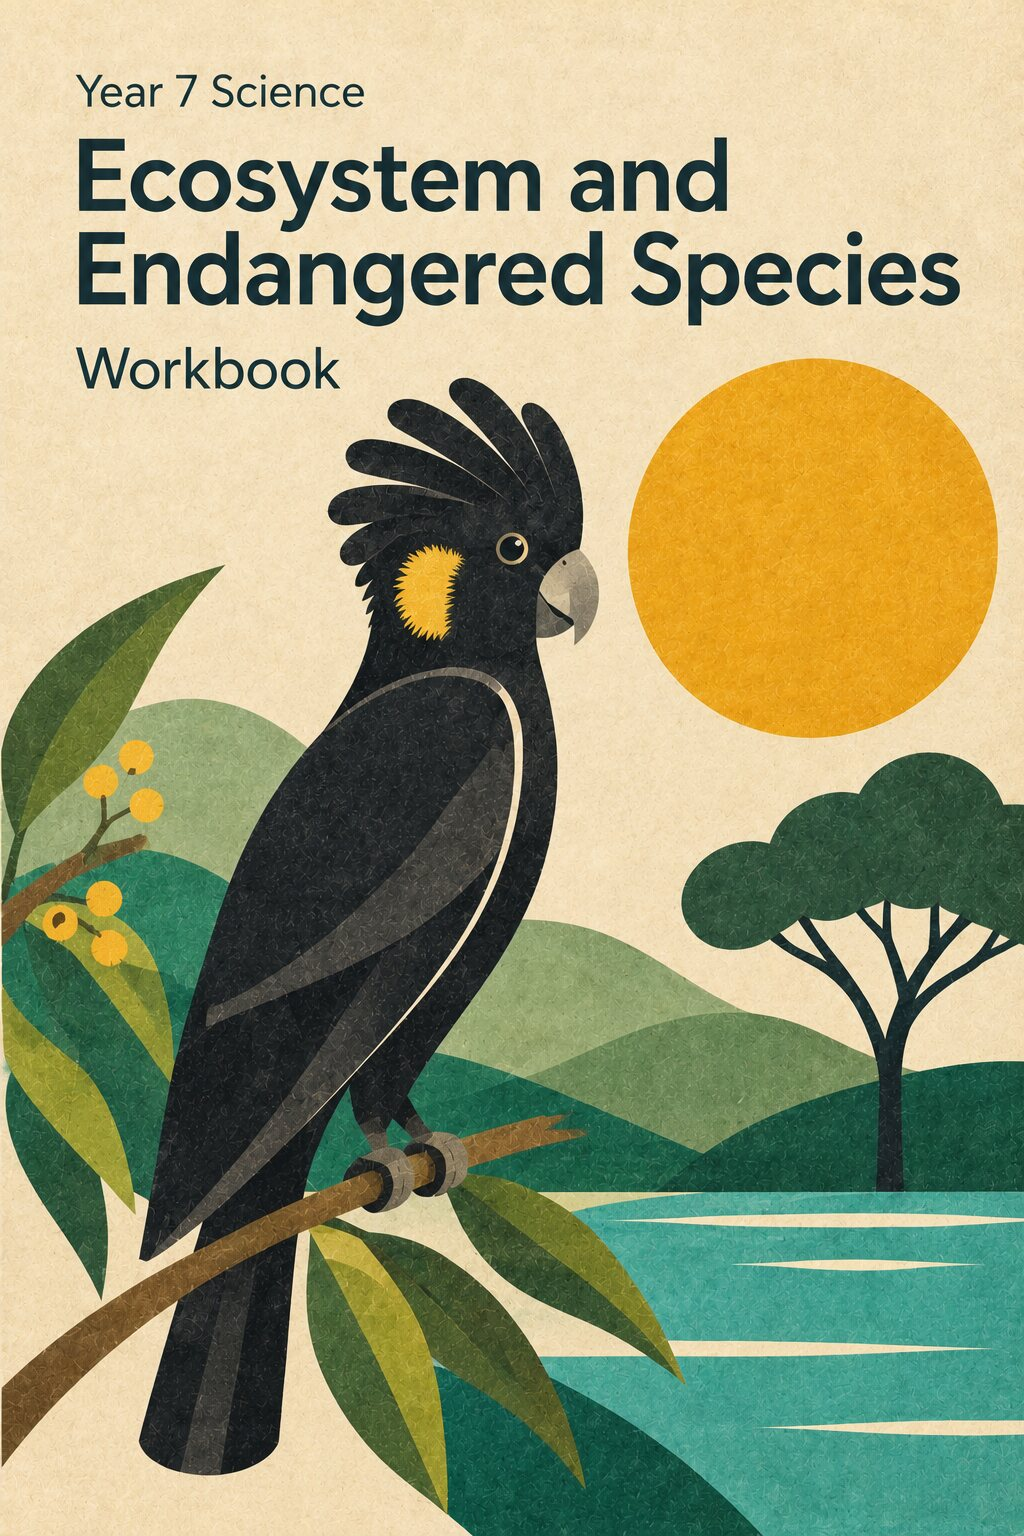
\includegraphics[width=\paperwidth]{../../../covers/ecosystems.jpg}};
  \node[anchor=north east, fill=white, draw=Ink, line width=0.6pt, rounded corners=1.2mm,
        inner xsep=2mm, inner ysep=1.8mm, text width=30mm, font=\headingfont\footnotesize]
    at ([xshift=-4mm, yshift=-4mm]current page.north east)
    {\textbf{Name}\par\vspace{4mm}\hrule\vspace{2mm}\textbf{Class}\par\vspace{4mm}\hrule};
  \node[anchor=south east, fill=white, draw=Ink, line width=0.6pt, rounded corners=1.2mm,
        inner xsep=2.6mm, inner ysep=2mm, font=\headingfont\bfseries, align=right]
    at ([xshift=-4mm, yshift=6mm]current page.south east)
    {Advanced Ecosystems 1\\[-1pt]{\normalfont\headingfont\scriptsize Topics 1--4}};
\end{tikzpicture}
\mbox{}
\clearpage

% ---- Inside cover ---------------------------------------------------------
\thispagestyle{plain}
{\headingfont\bfseries\fontsize{22}{26}\selectfont Advanced Ecosystems}\par\vspace{1mm}
{\headingfont\large Book 1 \textbullet\ Topics 1--4 \textbullet\ Above the Year 7 level}\par\vspace{1mm}
{\small\itshape VC 2.0: VC2S8U01--U04 \textbullet\ VC2S10U04 \textbullet\ VC2S10U05 \textbullet\ VC2S10U10}\par\vspace{4mm}
\textbf{Teacher}\ \hrulefill\par

\begin{countrybox}{Acknowledgement of Country}
This booklet was created on the unceded Country of the Wurundjeri Woi-wurrung people of the Kulin Nation. We acknowledge Elders past, present and emerging.
\end{countrybox}

\begin{infobox}{How this booklet works}
\textbf{Advanced Ecosystems} goes deeper into the ideas of the lesson books: more powerful models, the reasoning behind them, and harder problems that bring several ideas together. Each topic builds on the lessons named under its title. Each opens with its key vocabulary, then:\par\smallskip
\renewcommand{\arraystretch}{1.25}
\begin{tabular}{@{}p{24mm}p{70mm}@{}}
\textbf{Part A} & a reading with comprehension questions \\
\textbf{Part B} & the deeper idea, worked through \\
\textbf{Part C} & practice on your own \\
\textbf{Part D} & a challenge that pulls the ideas together \\
\end{tabular}

\smallskip
\begin{tabular}{@{}p{24mm}p{70mm}@{}}
\textbf{I do} \tagicon{\icodots{1}} & a worked example (solid frame) \\
\textbf{We do} \tagicon{\icodots{2}} & you try one with help (dashed frame) \\
\textbf{Reading} \tagicon{\icoread} & a passage to read (thin frame) \\
\end{tabular}
\end{infobox}

\clearpage
\markboth{Contents}{Contents}
{\headingfont\bfseries\LARGE Contents}\par\vspace{1mm}\noindent\rule{\linewidth}{0.6pt}\par\vspace{2mm}
\renewcommand{\arraystretch}{1.45}
\begin{tabular}{|C{1.1cm}|L{5.2cm}|C{1.7cm}|C{1.4cm}|}
  \hline\thead{Topic} & \thead{Title} & \thead{Deepens lesson} & \thead{Page} \\ \hline
  1 & \hyperlink{lesson.1.1}{Cells: the Units of Life} & 1 & \hyperlink{lesson.1.1}{p.\ \pageref{sec:1}} \\ \hline
  2 & \hyperlink{lesson.2.1}{The Tree of Life: Domains and DNA} & 2, 3 & \hyperlink{lesson.2.1}{p.\ \pageref{sec:2}} \\ \hline
  3 & \hyperlink{lesson.3.1}{What Is a Species? Keys and DNA Barcodes} & 4 & \hyperlink{lesson.3.1}{p.\ \pageref{sec:3}} \\ \hline
  4 & \hyperlink{lesson.4.1}{Measuring Biodiversity} & 5 & \hyperlink{lesson.4.1}{p.\ \pageref{sec:4}} \\ \hline
  5 & \textit{Energy Flow and the Carbon Cycle} & 6, 7 & Book 2 \\ \hline
  6 & \textit{Natural Selection and Evolution} & 8 & Book 2 \\ \hline
  7 & \textit{Populations, Invaders and Extinction} & 9, 10, 11 & Book 2 \\ \hline
  --- & \hyperlink{glossary}{Glossary} & & \hyperlink{glossary}{\pageref{sec:glossary}} \\ \hline
\end{tabular}
\renewcommand{\arraystretch}{1}
\clearpage
\setcounter{section}{0}\renewcommand{\lessonart}{1}
\sectiondiv{Cells: the Units of Life}{Cell theory \textbullet{} Plant and animal cells \textbullet{} Magnification \textbullet{} Why cells are small}\label{sec:1}
\lessoncodes{Deepens Lesson 1 \textbullet{} VC2S8U02 \textbullet{} VC2S8U03}

\vocabhead
\begin{ctab}
\begin{tabular}{|SW{3.4cm}|W{7.0cm}|}
  \hline\hd & \thead{Word} & \thead{Definition (copy from the slide)} \\ \hline
  & \scaf{\textbf{Cell}\label{voc:cell}} & \scaf{The smallest unit that can carry out all the processes of life.} \\ \hline
  & \textbf{Cell theory}\label{voc:cell-theory} & \\ \hline
  & \textbf{Organelle}\label{voc:organelle} & \\ \hline
  & \textbf{Nucleus}\label{voc:nucleus} & \\ \hline
  & \textbf{Chloroplast}\label{voc:chloroplast} & \\ \hline
  & \textbf{Magnification}\label{voc:magnification} & \\ \hline
\end{tabular}
\end{ctab}

\lessonpart{A}{Reading and comprehension}{Teal}\label{read:1}

\begin{readingbox}{Reading --- Seeing the Invisible}
In 1665 Robert Hooke looked at a thin slice of cork through one of the first microscopes. He saw rows of tiny empty boxes and called them \emph{cells}, because they reminded him of the small rooms monks lived in. A few years later Antonie van Leeuwenhoek, using lenses he ground himself, saw living ``animalcules'' swimming in pond water: the first people ever to see bacteria and single-celled organisms.

Nearly two hundred years later, scientists put the evidence together into \textbf{cell theory}: every living thing is made of one or more cells; the cell is the smallest unit of life; and every cell comes from a cell that already existed. A bacterium is a single cell. You are about 37 trillion of them, working together.

Inside a cell are smaller parts with their own jobs, called \textbf{organelles}. The \textbf{nucleus} holds the cell's DNA, the instructions for building and running it. Plant cells also have \textbf{chloroplasts}, where light energy is captured to make food.

Most cells are far too small to see. A light microscope makes them look bigger: its \textbf{magnification} tells you how many times bigger the image is than the real thing.
\end{readingbox}

\rcreset
\rcq{What did Hooke see in cork, and why did he call them cells?}{2.5cm}
\rcq{State the three ideas of cell theory.}{3cm}
\rcq{What is an organelle? Give two examples and their jobs.}{2.5cm}
\rcq{Why could nobody study cells before the 1600s?}{2cm}

\lessonpart{B}{Theory and examples}{Blue}\label{theory:1}

\subsection{Plant and Animal Cells}\label{sub:a1.1}

\begin{ctab}
\begin{tabular}{|C{3.0cm}|C{1.5cm}|C{1.5cm}|W{4.0cm}|}
  \hline\thead{Part} & \thead{Animal} & \thead{Plant} & \thead{Job} \\ \hline
  Cell membrane & yes & yes & controls what enters and leaves \\ \hline
  Cytoplasm & yes & yes & jelly where most reactions happen \\ \hline
  Nucleus & yes & yes & holds the DNA; controls the cell \\ \hline
  Mitochondria & yes & yes & release energy from food (respiration) \\ \hline
  Cell wall & no & yes & stiff outer layer that supports the cell \\ \hline
  Chloroplasts & no & yes & capture light to make food (photosynthesis) \\ \hline
  Large vacuole & no & yes & stores water and keeps the cell firm \\ \hline
\end{tabular}
\end{ctab}

\begin{workedex}{Plant or animal?}
A cell from a leaf of a pondweed has a nucleus, a cell wall, a large vacuole and many small green discs.

\smallskip
It is a \textbf{plant} cell. The cell wall and large vacuole are found only in plant cells, and the green discs are chloroplasts, which make food by photosynthesis.
\end{workedex}

\begin{wedo}{Plant or animal?}
A cell scraped from the inside of a cheek has a nucleus, a cell membrane and cytoplasm, but no cell wall and no chloroplasts. A cell from an onion bulb has a cell wall and a large vacuole but no chloroplasts. Identify each cell, and explain why the onion cell has no chloroplasts even though it is a plant cell.
\answerbox{5cm}
\end{wedo}

\subsection{Magnification}\label{sub:a1.2}

\begin{skillbox}{Magnification}
\[ \text{magnification} = \frac{\text{image size}}{\text{actual size}} \]
Both sizes must be in the same unit. Cells are measured in micrometres (\textmu m): $1\,\text{mm} = 1000\,\text{\textmu m}$.
\end{skillbox}

\begin{workedex}{Finding the magnification}
A cheek cell is 60\,\textmu m across. In a photograph it measures 30\,mm. Find the magnification.

\smallskip
Same units first: $30\,\text{mm} = 30 \times 1000 = 30\,000\,\text{\textmu m}$.\\
Magnification $= 30\,000 \div 60 = \mathbf{500\times}$.
\end{workedex}

\begin{wedo}{Finding the actual size}
A photograph of a red blood cell taken at $\times 2000$ shows the cell as 16\,mm across. Find the actual width of the cell in micrometres. (Rearrange: actual size $=$ image size $\div$ magnification.)
\workbox{4.5cm}
\end{wedo}

\lessonpart{C}{Practice}{Amber}\label{prac:1}

\begin{keepext}
\task Plant cells and animal cells both carry out all seven life processes. Describe two parts of a plant cell that an animal cell does not have, and explain how one of them lets a plant make its own food.
\answerbox{5cm}
\end{keepext}
\begin{keepext}
\task Some scientists argue that viruses should count as living, because they change over time and carry genetic material. Give one piece of evidence for and one against this argument, and state your own view.
\answerbox{5cm}
\end{keepext}


\needspace{10\baselineskip}
\task A leaf cell is 0.1\,mm long. Calculate how long it would appear under a microscope set to $\times 400$, in millimetres.
\workbox{4cm}

\lessonpart{D}{Challenge}{Violet}\label{ext:1}

\task Why are cells so small? A cell takes in food and oxygen through its surface, but uses them throughout its volume.
\pt{a} Calculate the surface area and the volume of a cube of side 1\,cm and a cube of side 3\,cm, and the surface area to volume ratio of each.
\workbox{6cm}
\pt{b} Use your answers to explain why a large organism is made of many small cells instead of one huge cell.
\answerbox{5cm}

\clearpage

% ══════════════════════════════════════════════════════════════════════════════
%  TOPIC 2 — THE TREE OF LIFE: DOMAINS AND DNA          (deepens Lessons 2, 3)
% ══════════════════════════════════════════════════════════════════════════════
\setcounter{section}{1}\renewcommand{\lessonart}{2}
\sectiondiv{The Tree of Life: Domains and DNA}{Three domains \textbullet{} Prokaryotes and eukaryotes \textbullet{} Reading an evolutionary tree \textbullet{} DNA evidence}\label{sec:2}
\lessoncodes{Deepens Lessons 2 and 3 \textbullet{} VC2S8U01 \textbullet{} VC2S10U04 \textbullet{} VC2S10U05}

\vocabhead
\begin{ctab}
\begin{tabular}{|SW{3.4cm}|W{7.0cm}|}
  \hline\hd & \thead{Word} & \thead{Definition (copy from the slide)} \\ \hline
  & \scaf{\textbf{Domain}\label{voc:domain}} & \scaf{The largest group in classification, above kingdom. There are three: Bacteria, Archaea and Eukarya.} \\ \hline
  & \textbf{Prokaryote}\label{voc:prokaryote} & \\ \hline
  & \textbf{Eukaryote}\label{voc:eukaryote} & \\ \hline
  & \textbf{Common ancestor}\label{voc:common-ancestor} & \\ \hline
  & \textbf{Evolutionary tree}\label{voc:evolutionary-tree} & \\ \hline
  & \textbf{DNA sequence}\label{voc:dna-sequence} & \\ \hline
\end{tabular}
\end{ctab}

\lessonpart{A}{Reading and comprehension}{Teal}\label{read:2}

\begin{readingbox}{Reading --- The Microbes That Rewrote the Tree}
For most of the 1900s, scientists sorted every tiny single-celled organism without a nucleus into one group: bacteria. Cells like these, with their DNA loose in the cytoplasm, are \textbf{prokaryotes}. Cells with a nucleus, like ours, are \textbf{eukaryotes}.

In 1977 the American scientist Carl Woese compared not what microbes looked like, but the order of the chemical ``letters'' in one of their genes: their \textbf{DNA sequence}. Some microbes from hot springs and salty lakes turned out to be as different from bacteria, in their genes, as bacteria are from us. Woese named them Archaea and proposed a new top level of classification: three \textbf{domains}, Bacteria, Archaea and Eukarya. Many scientists thought he was wrong. Today his three domains are in every textbook.

DNA changes slowly over many generations. Two species that split from a \textbf{common ancestor} recently have had little time to build up differences, so their DNA is very alike. Species that split long ago differ more. Scientists use these differences to draw an \textbf{evolutionary tree}: a diagram showing which groups share the most recent ancestors.
\end{readingbox}

\rcreset
\rcq{What is the difference between a prokaryote and a eukaryote?}{2.5cm}
\rcq{What evidence did Woese use, and why was it new?}{2.5cm}
\rcq{Why were many scientists slow to accept the three domains? What made them change their minds?}{3cm}
\rcq{Why do closely related species have very similar DNA?}{2.5cm}

\lessonpart{B}{Theory and examples}{Blue}\label{theory:2}

\subsection{Three Domains}\label{sub:a2.1}

\begin{ctab}
\begin{tabular}{|C{2.3cm}|W{2.6cm}|W{5.3cm}|}
  \hline\thead{Domain} & \thead{Cell type} & \thead{Examples} \\ \hline
  Bacteria & prokaryote & \textit{E.\ coli}, the bacteria in yoghurt and in soil \\ \hline
  Archaea & prokaryote & microbes of hot springs, salt lakes and animal guts \\ \hline
  Eukarya & eukaryote & every protist, fungus, plant and animal \\ \hline
\end{tabular}
\end{ctab}

\begin{workedex}{Placing an organism}
A microbe found in the salt lakes of the Victorian Mallee has no nucleus, and its genes are unlike those of any bacterium.

\smallskip
No nucleus means it is a prokaryote, so it is in Bacteria or Archaea. Its genes are unlike any bacterium's, so it belongs in \textbf{Archaea}. Its home, a salty lake, is typical of archaea, but the genes are the deciding evidence.
\end{workedex}

\begin{wedo}{Placing an organism}
Place each in a domain and give your reason: a mushroom; the bacterium that turns milk into yoghurt; a single-celled algae with a nucleus and a chloroplast.
\answerbox{4.5cm}
\end{wedo}

\subsection{Reading an Evolutionary Tree}\label{sub:a2.2}

\begin{center}
\begin{fitbox}\begin{tikzpicture}[font=\small, line width=0.9pt]
  \draw (0,0) -- (1,0);
  \draw (1,0) -- (1,1.5) -- (6,1.5) node[right] {platypus};
  \draw (1,0) -- (1,-0.75) -- (3,-0.75);
  \draw (3,-0.75) -- (3,0.25) -- (6,0.25) node[right] {human};
  \draw (3,-0.75) -- (3,-1.5) -- (4.5,-1.5);
  \draw (4.5,-1.5) -- (4.5,-0.9) -- (6,-0.9) node[right] {koala};
  \draw (4.5,-1.5) -- (4.5,-2.1) -- (6,-2.1) node[right] {kangaroo};
  \fill (1,0) circle (2pt) (3,-0.75) circle (2pt) (4.5,-1.5) circle (2pt);
  \node[below left, font=\scriptsize] at (1,0) {A};
  \node[below left, font=\scriptsize] at (3,-0.75) {B};
  \node[below left, font=\scriptsize] at (4.5,-1.5) {C};
  \draw[->, line width=0.6pt] (0,-2.6) -- (6,-2.6) node[midway, below, font=\scriptsize] {time: past to present};
\end{tikzpicture}\end{fitbox}
\figcap{Each dot is a common ancestor. The later two groups split, the more closely they are related.}
\end{center}

\begin{workedex}{Who is more closely related?}
Is the koala more closely related to the kangaroo or to the human?

\smallskip
The koala and kangaroo share ancestor C. The koala and human only share ancestor B, which lived earlier. So the koala is \textbf{more closely related to the kangaroo}: they split from each other more recently.
\end{workedex}

\begin{wedo}{Who is more closely related?}
Use the tree. Is the human more closely related to the kangaroo or to the platypus? Which ancestor do all four share?
\answerbox{4cm}
\end{wedo}

\lessonpart{C}{Practice}{Amber}\label{prac:2}

\begin{keepext}
\task Scientists now place three \textbf{domains} above the kingdoms: Bacteria, Archaea and Eukarya. Explain what feature of the cells separates the domains, then place each of these in a domain: a human, the bacterium \textit{E.\ coli}, a microbe from a hot spring (\textit{Sulfolobus}).
\answerbox{5cm}
\end{keepext}
\begin{keepext}
\task Reading DNA has moved some organisms to different groups. Explain why DNA evidence is more reliable than appearance for working out how closely organisms are related.
\answerbox{5cm}
\end{keepext}


\begin{keepext}
\task Fungi were once classified as plants. Describe two features of fungi that make them different from plants, and explain why these justify a separate kingdom.
\answerbox{5cm}
\end{keepext}
\begin{keepext}
\task Draw and label a simple prokaryotic cell and a simple eukaryotic cell, showing the key difference between them.
\drawbox{5.5cm}{}
\end{keepext}


\lessonpart{D}{Challenge}{Violet}\label{ext:2}

\task Scientists compared 100 letters of the same gene in four species, W, X, Y and Z. The table shows how many letters differ between each pair.
\begin{ctab}
\begin{tabular}{|C{1.4cm}|C{1.4cm}|C{1.4cm}|C{1.4cm}|C{1.4cm}|}
  \hline & \thead{W} & \thead{X} & \thead{Y} & \thead{Z} \\ \hline
  \thead{W} & --- & 3 & 11 & 19 \\ \hline
  \thead{X} & 3 & --- & 12 & 19 \\ \hline
  \thead{Y} & 11 & 12 & --- & 20 \\ \hline
  \thead{Z} & 19 & 19 & 20 & --- \\ \hline
\end{tabular}
\end{ctab}
\pt{a} Which two species are most closely related? Which species split off from the others first?
\answerbox{3cm}
\pt{b} Draw an evolutionary tree for the four species, like the one in Part B.
\drawbox{6cm}{}

\clearpage

% ══════════════════════════════════════════════════════════════════════════════
%  TOPIC 3 — WHAT IS A SPECIES? KEYS AND DNA BARCODES        (deepens Lesson 4)
% ══════════════════════════════════════════════════════════════════════════════
\setcounter{section}{2}\renewcommand{\lessonart}{4}
\sectiondiv{What Is a Species? Keys and DNA Barcodes}{Defining a species \textbullet{} Hybrids \textbullet{} Writing a key that works \textbullet{} DNA barcoding}\label{sec:3}
\lessoncodes{Deepens Lesson 4 \textbullet{} VC2S8U01 \textbullet{} VC2S10I06}

\vocabhead
\begin{ctab}
\begin{tabular}{|SW{3.4cm}|W{7.0cm}|}
  \hline\hd & \thead{Word} & \thead{Definition (copy from the slide)} \\ \hline
  & \scaf{\textbf{Fertile}\label{voc:fertile}} & \scaf{Able to produce young of its own.} \\ \hline
  & \textbf{Hybrid}\label{voc:hybrid} & \\ \hline
  & \textbf{Cryptic species}\label{voc:cryptic-species} & \\ \hline
  & \textbf{Couplet}\label{voc:couplet} & \\ \hline
  & \textbf{DNA barcode}\label{voc:dna-barcode} & \\ \hline
\end{tabular}
\end{ctab}

\lessonpart{A}{Reading and comprehension}{Teal}\label{read:3}

\begin{readingbox}{Reading --- One Species or Two?}
The usual definition says a species is a group of organisms that can breed together and have \textbf{fertile} young. It works well for most animals. A horse and a donkey can breed, but their young, a mule, is almost always sterile, so horses and donkeys are separate species. A mule is a \textbf{hybrid}: the young of two different species.

But the definition has problems. Bacteria do not breed in pairs at all. Fossils cannot be tested for breeding. Some plants form fertile hybrids easily. And some animals look identical but never breed together: they are \textbf{cryptic species}, hidden from anyone who only looks. Frogs that look the same but have different calls are a common example.

Because of this, scientists now use several lines of evidence together: appearance, behaviour, where the organism lives, and its DNA. A short, standard stretch of an animal's DNA can work like the barcode on a packet in a supermarket. Comparing this \textbf{DNA barcode} against a library of known species can name an organism from a single hair, a scale or a scrap of leaf.
\end{readingbox}

\rcreset
\rcq{Why are horses and donkeys separate species, even though they can breed?}{2.5cm}
\rcq{Give two kinds of organism the breeding definition does not work for, and why.}{3cm}
\rcq{What is a cryptic species, and how might scientists discover one?}{2.5cm}
\rcq{Why can a DNA barcode identify an organism a key cannot?}{2.5cm}

\lessonpart{B}{Theory and examples}{Blue}\label{theory:3}

\subsection{Writing a Key That Works}\label{sub:a3.1}

\begin{skillbox}{Rules for a good couplet}
Each step of a key is a \textbf{couplet}: two statements, and every organism must fit exactly one.
\textbf{1.} Use features anyone can see on any adult of the species. \textbf{2.} Make the two halves opposites (``has a pouch'' / ``has no pouch''). \textbf{3.} Avoid size, colour and ``big or small'', which vary between individuals. \textbf{4.} Split the group, roughly in half if you can.
\end{skillbox}

\begin{workedex}{Fixing a weak couplet}
\textbf{Weak:} 1a.\ Large brown bird \qquad 1b.\ Small bird with a long tail

\smallskip
``Large'' and ``small'' depend on what you compare them with, a young bird may be small, and the two halves describe different features (colour, tail), so a small brown bird with a short tail fits neither.
\textbf{Better:} 1a.\ Tail longer than body \qquad 1b.\ Tail shorter than body.
\end{workedex}

\begin{wedo}{Fixing a weak couplet}
Rewrite this couplet so it follows all four rules: 2a.\ Green frog with spots \qquad 2b.\ Brown frog that is good at climbing.
\answerbox{4cm}
\end{wedo}

\subsection{Is It a Separate Species?}\label{sub:a3.2}

\begin{workedex}{Using several lines of evidence}
Two populations of tree frog in eastern Victoria look the same. Females only move towards the call of their own population, and their DNA barcodes differ by 6\%. (Individuals of one species usually differ by less than 2\%.)

\smallskip
They do not breed together, because the females choose different calls, and their DNA is far more different than within one species. Both lines of evidence say they are \textbf{two cryptic species}.
\end{workedex}

\begin{wedo}{Using several lines of evidence}
Lions and tigers do not meet in the wild. In zoos they can breed, and their young (ligers) are usually sterile. Decide whether lions and tigers are one species or two, and use two lines of evidence.
\answerbox{4.5cm}
\end{wedo}

\lessonpart{C}{Practice}{Amber}\label{prac:3}

\begin{keepext}
\task Keys go wrong when members of one species look different: young and adults, or males and females. Describe how this could make a key give the wrong answer, and suggest how to improve the key.
\answerbox{5cm}
\end{keepext}
\begin{keepext}
\task DNA barcoding identifies a species from a short piece of its DNA. A scientist finds an unknown beetle in a Victorian forest. Give one advantage and one limitation of DNA barcoding compared with a dichotomous key.
\answerbox{5cm}
\end{keepext}


\lessonpart{D}{Challenge}{Violet}\label{ext:3}

\task Write a dichotomous key that identifies these six Australian animals. Use only features in the table, follow the four rules, and use five couplets.
\begin{ctab}
\begin{tabular}{|W{2.5cm}|C{1.6cm}|C{1.5cm}|C{1.5cm}|C{1.5cm}|}
  \hline\thead{Animal} & \thead{Body covering} & \thead{Lays eggs} & \thead{Pouch} & \thead{Wings} \\ \hline
  Platypus & fur & yes & no & no \\ \hline
  Echidna & fur and spines & yes & yes & no \\ \hline
  Koala & fur & no & yes & no \\ \hline
  Dingo & fur & no & no & no \\ \hline
  Kookaburra & feathers & yes & no & yes \\ \hline
  Blue-tongue lizard & scales & no & no & no \\ \hline
\end{tabular}
\end{ctab}
\answerbox{8cm}

\clearpage

% ══════════════════════════════════════════════════════════════════════════════
%  TOPIC 4 — MEASURING BIODIVERSITY                          (deepens Lesson 5)
% ══════════════════════════════════════════════════════════════════════════════
\setcounter{section}{3}\renewcommand{\lessonart}{5}
\sectiondiv{Measuring Biodiversity}{Sampling \textbullet{} Richness and evenness \textbullet{} Simpson's index \textbullet{} Capture--recapture}\label{sec:4}
\lessoncodes{Deepens Lesson 5 \textbullet{} VC2S8U04 \textbullet{} VC2S10I03 \textbullet{} VC2S10I04}

\vocabhead
\begin{ctab}
\begin{tabular}{|SW{3.4cm}|W{7.0cm}|}
  \hline\hd & \thead{Word} & \thead{Definition (copy from the slide)} \\ \hline
  & \scaf{\textbf{Sample}\label{voc:sample}} & \scaf{A small part of an area or population, studied to estimate what the whole is like.} \\ \hline
  & \textbf{Species richness}\label{voc:species-richness} & \\ \hline
  & \textbf{Species evenness}\label{voc:species-evenness} & \\ \hline
  & \textbf{Diversity index}\label{voc:diversity-index} & \\ \hline
  & \textbf{Capture--recapture}\label{voc:capture-recapture} & \\ \hline
\end{tabular}
\end{ctab}

\lessonpart{A}{Reading and comprehension}{Teal}\label{read:4}

\begin{readingbox}{Reading --- Counting What You Cannot See}
How many skinks live in a grassland? Nobody can find every one. Ecologists study a \textbf{sample} instead: a few quadrats, a line of pitfall traps, or a set of camera traps, chosen so they represent the whole area. Then they scale up.

Counting species is only half the story. \textbf{Species richness} is the number of species. \textbf{Species evenness} is how equal their numbers are. Imagine two paddocks, each with four plant species and 100 plants. In the first, there are 25 of each. In the second, there are 97 of one weed and one each of the others. They have the same richness, but the first is far more diverse, because no single species dominates.

A \textbf{diversity index} combines richness and evenness into one number, so places can be compared fairly. For animals that move, ecologists use \textbf{capture--recapture}: they catch some animals, mark them harmlessly, release them, then catch again later. The share of marked animals in the second catch reveals how big the whole population is.
\end{readingbox}

\rcreset
\rcq{Why do ecologists sample instead of counting every organism?}{2.5cm}
\rcq{Explain the difference between species richness and species evenness.}{2.5cm}
\rcq{Which of the two paddocks in the reading has higher biodiversity, and why?}{2.5cm}
\rcq{Why must a sample be chosen to represent the whole area?}{2.5cm}

\lessonpart{B}{Theory and examples}{Blue}\label{theory:4}

\subsection{Simpson's Diversity Index}\label{sub:a4.1}

\begin{skillbox}{Simpson's index}
\[ D = 1 - \sum\left(\frac{n}{N}\right)^2 \]
$n$ is the number of one species, $N$ the total of all organisms. Work out $\frac{n}{N}$ for every species, square each one, add them up, and take the total away from 1. $D$ runs from 0 (one species only) towards 1 (many species, evenly spread).
\end{skillbox}

\begin{workedex}{Calculating $D$}
A quadrat holds 20 plants: 6 wallaby grass, 6 kangaroo grass, 6 daisies and 2 orchids.

\smallskip
$\frac{n}{N}$: $\ 0.3,\ 0.3,\ 0.3,\ 0.1$ \quad squared: $\ 0.09,\ 0.09,\ 0.09,\ 0.01$\\
Sum $= 0.28$, so $D = 1 - 0.28 = \mathbf{0.72}$: a fairly diverse quadrat.
\end{workedex}

\begin{wedo}{Calculating $D$}
A quadrat holds 20 plants: 8 of species P, 8 of species Q and 4 of species R. Calculate $D$, and say whether it is more or less diverse than the worked example.
\workbox{5cm}
\end{wedo}

\subsection{Capture--Recapture}\label{sub:a4.2}

\begin{skillbox}{Estimating a population}
\[ \text{population} \approx \frac{\text{number marked} \times \text{number caught second time}}{\text{number of marked animals recaught}} \]
It assumes marks do not fall off or harm the animal, marked animals mix back in, and no animals are born, die or move in between the two catches.
\end{skillbox}

\begin{workedex}{Estimating a population}
Ecologists catch and mark 30 skinks. A week later they catch 40, and 8 of them are marked.

\smallskip
Population $\approx \dfrac{30 \times 40}{8} = \dfrac{1200}{8} = \mathbf{150}$ skinks.
\end{workedex}

\begin{wedo}{Estimating a population}
Rangers mark 20 eastern barred bandicoots. Two weeks later they trap 25, and 5 are marked. Estimate the population, and give one reason the estimate could be wrong.
\workbox{5cm}
\end{wedo}

\lessonpart{C}{Practice}{Amber}\label{prac:4}

\begin{keepext}
\task Simpson's diversity index is $D = 1 - \sum\left(\dfrac{n}{N}\right)^2$, where $n$ is the number of each species and $N$ is the total. Quadrat A has 20 organisms of four species (10, 5, 3, 2); quadrat B has 20 organisms of two species (18, 2). Calculate $D$ for each and explain what the values mean.
\workbox{6cm}
\end{keepext}
\begin{keepext}
\task Explain why genetic diversity within a species helps it survive a new disease.
\answerbox{5cm}
\end{keepext}


\needspace{10\baselineskip}
\task Ten 1\,m$^2$ quadrats in a 2000\,m$^2$ grassland hold 3, 5, 2, 4, 0, 6, 3, 4, 5 and 2 orchids. Estimate the number of orchids in the whole grassland. Show your working.
\workbox{5cm}

\lessonpart{D}{Challenge}{Violet}\label{ext:4}

\task In a capture--recapture study, the marked animals learn that the traps hold food, and walk into them more readily the second time.
\pt{a} Will the number of marked animals recaught be too high or too low? Explain.
\answerbox{3.5cm}
\pt{b} Will the population estimate be too high or too low? Use the formula to explain.
\answerbox{3.5cm}
\pt{c} Suggest a change to the method that would reduce the problem.
\answerbox{3cm}

\clearpage

% ══════════════════════════════════════════════════════════════════════════════
%  TOPIC 5 — ENERGY FLOW AND THE CARBON CYCLE           (deepens Lessons 6, 7)
% ══════════════════════════════════════════════════════════════════════════════

\clearpage\markboth{Glossary}{Glossary}\hypertarget{glossary}{}\pdfbookmark[1]{Glossary}{glossarybm}
{\headingfont\bfseries\LARGE Glossary}\label{sec:glossary}\par\vspace{1mm}\noindent\rule{\linewidth}{0.6pt}\par
{\small Every key word in this booklet and the page it is introduced on.}\par\smallskip
\renewcommand{\arraystretch}{1.3}
\begin{longtable}{|>{\RaggedRight}p{34mm}|p{9mm}|p{\dimexpr\linewidth-43mm-6\tabcolsep-4\arrayrulewidth-1pt\relax}|}
\hline \rule{0pt}{4mm}\headingfont\bfseries Word & \headingfont\bfseries Page & \headingfont\bfseries In my own words \\ \hline \endhead
  Capture--recapture & \pageref{voc:capture-recapture} & \\ \hline
  Cell & \pageref{voc:cell} & \\ \hline
  Cell theory & \pageref{voc:cell-theory} & \\ \hline
  Chloroplast & \pageref{voc:chloroplast} & \\ \hline
  Common ancestor & \pageref{voc:common-ancestor} & \\ \hline
  Couplet & \pageref{voc:couplet} & \\ \hline
  Cryptic species & \pageref{voc:cryptic-species} & \\ \hline
  Diversity index & \pageref{voc:diversity-index} & \\ \hline
  DNA barcode & \pageref{voc:dna-barcode} & \\ \hline
  DNA sequence & \pageref{voc:dna-sequence} & \\ \hline
  Domain & \pageref{voc:domain} & \\ \hline
  Eukaryote & \pageref{voc:eukaryote} & \\ \hline
  Evolutionary tree & \pageref{voc:evolutionary-tree} & \\ \hline
  Fertile & \pageref{voc:fertile} & \\ \hline
  Hybrid & \pageref{voc:hybrid} & \\ \hline
  Magnification & \pageref{voc:magnification} & \\ \hline
  Nucleus & \pageref{voc:nucleus} & \\ \hline
  Organelle & \pageref{voc:organelle} & \\ \hline
  Prokaryote & \pageref{voc:prokaryote} & \\ \hline
  Sample & \pageref{voc:sample} & \\ \hline
  Species evenness & \pageref{voc:species-evenness} & \\ \hline
  Species richness & \pageref{voc:species-richness} & \\ \hline
\end{longtable}
\padtofour
\end{document}
